\section{An\'alisis te\'orico del circuito}

	\subsection{Polarizaci\'on}
		
		\begin{figure}[H]
			\centering
			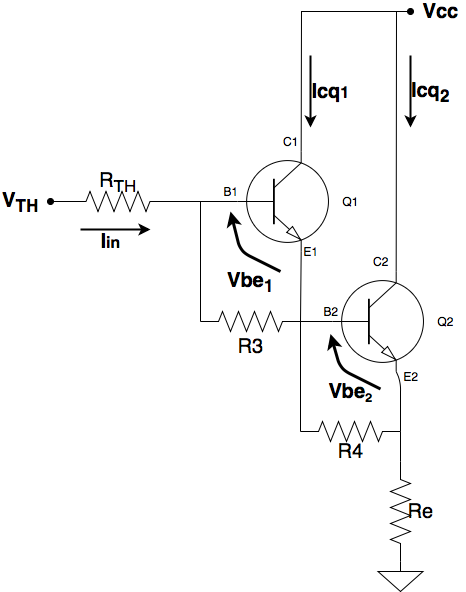
\includegraphics[scale=0.4]{./Imagenes/polarizacion.png} \\
			\caption{Circuito equivalente para el an\'alisis de polarizaci\'on.}
			\label{polarizacion}
		\end{figure}

	\begin{equation}	
		\begin{cases}
		V_{TH} = \frac{R_2}{R_1 + R_2} V_{CC}\\ \\
		R_{TH} = R_1 // R_2
		\end{cases}
		\label{Thevenin}
	\end{equation}
	
	\begin{equation}
	\begin{cases}
		V_{TH} -  R_{TH} I_{TH} - Vbe_1 - Vbe_2 -(Ie_2 + I_{R4})Re = 0\\ \\
		I_{TH} = Ib_1 + \frac{Vbe_1}{R_3}\\ \\
		Ie_2 = (HFE_2 + 1)Ib_2\\ \\
		Ib_2 = \frac{Vbe_1}{R_3} + (HFE_1+1)Ib_1 - \frac{Vbe_2}{R_4}
		\end{cases}
	\end{equation}
	
		\begin{equation}
	\begin{cases}
	Ic_1 = (HFE_1 + 1)Ib_1\\ \\
	Ic_2 = HFE_2 (\frac{Vbe_1}{R_3} + (HFE_1 + 1)Ib_1 - \frac{Vbe_2}{R_4})
	\end{cases}
	\end{equation}
	
	\todo{Seguir pasando en limpio las ecs de polarizacion y explicar paso a paso}

	\subsection{Modelo incremental}
	
		\begin{equation}
			\begin{cases}
			\widehat{r}_{aux} = \frac{V_T}{I_{cq}}\\
			\widehat{g}_m = \frac{1}{r_{aux}}\\	
			\widehat{h}_{ie} = (h_{fe} + 1) r_{aux}\\
			\widehat{r}_{ce} = \frac{1}{h_{oe}} = \frac{V_A}{I_{cq}}
			\end{cases}
			\label{mod_inc_ecs}
		\end{equation}
	
	Particularmente, para el transistor $Q1$ se emplean las ecuaciones \ref{mod_inc_ecs} con $I_{cq1}$ y $h_{fe1}$, mientras que para el transistor $Q2$ con $I_{cq2}$ y $h_{fe2}$. Se obtienen los siguientes valores:
	
	\todo{COMPLETAR TABLA de estimadores}
	\begin{table}[h!]
		\centering
		\begin{tabular}{c c c}%
			\bfseries Estimadores & Q1 & Q2 \\ \hline
			$\widehat{g}_m$ &  & \\
			$\widehat{h}_{ie}$ &  & \\
			$\widehat{r}_{ce}$&  & \\
			\hline
		\end{tabular}
		\caption{Estimadores correspondientes al modelo incremental, para los transistores Q1 y Q2.}
		\label{avolf}
	\end{table}
	
	\subsection{Circuito incremental}
	
		\begin{figure}[H]
			\centering
			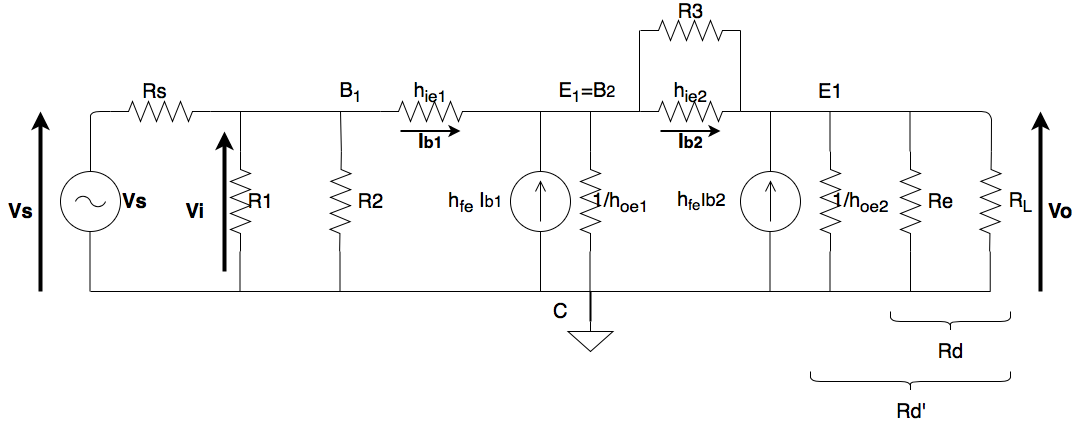
\includegraphics[scale=0.4]{./Imagenes/circ_incremental.png} \\
			\caption{Circuito equivalente para el an\'alisis del circuito incremental.}
			\label{circ_incremental}
		\end{figure}

\section{Diseño del circuito}